\documentclass[]{report}
\usepackage{geometry}
\usepackage{graphicx}
\usepackage{physics}
\usepackage{color}
\usepackage{subcaption}
\usepackage{lipsum}
\usepackage{amsmath}
\usepackage{amsfonts}
\usepackage{amssymb}
\usepackage[hidelinks]{hyperref}
\usepackage{parskip}
\usepackage{mathtools}
\usepackage{tikz}
\usepackage{bm}
\usetikzlibrary{shapes.callouts, shapes.geometric, arrows}
\tikzset{
	level/.style = {
		ultra thick,
		black,
	},
	connect/.style = {
		dashed,
		black
	},
	notice/.style = {
		draw,
		rectangle callout,
		callout relative pointer={#1}
	},
	label/.style = {
		text width=2cm
	}
}
\tikzstyle{arrow} = [<->,>=stealth]

\newcommand{\up}{\fbox{$\uparrow\phantom{\downarrow}$}}%
\newcommand{\dwn}{\fbox{$\phantom{\uparrow}\downarrow$}}%
\newcommand{\updwn}{\fbox{$\mathord\uparrow\downarrow$}}%
\newcommand{\emp}{\fbox{$\phantom{\downarrow}\phantom{\downarrow}$}}%
\newcommand{\electron}[2]{{%
		\setlength\tabcolsep{0pt}% remove extra horizontal space from tabular
		      %\setlength\fboxrule{0.2pt}% uncomment for original line width
		\begin{tabular}{c}
			\fboxsep=0pt\fbox{\fboxsep=3pt#2}\\[2pt]
			#1
		\end{tabular}%
}}

%\geometry{top = 2.5cm, bottom = 2.5cm, left = 2.5cm, right = 2.5cm}
%
\setlength{\parindent}{0mm}
%\setlength{\parskip}{0.5mm}

\renewcommand{\vec}{\bm}

% Title Page
\title{A Study of the t-J Model\vspace{-5mm}}
\author{Amit Bikram Sanyal}
\date{Submitted on \today}

\newcommand{\I}{\,\mathrm{i}\,}

%\let\cleardoublepage=\clearpage

\begin{document}
	
\begin{minipage}{\linewidth}
	\maketitle
\end{minipage}

\vfill

\begin{center}
	\includegraphics[width=0.4\linewidth]{images/niser-logo}
\end{center}


\newpage
\tableofcontents
\thispagestyle{empty}

\begin{abstract}
	\lipsum[1]
\end{abstract}

\chapter{The Hubbard model with strong interactions}
\section{Introduction}
The Hubbard model is one of the simplest many-body models. The one-dimensional model consists of an array of $ N $ sites with $ L $ fermions. The Hubbard model captures the effect of the electrons hopping from site to site, causing the electrons to de-localize and give rise to metallic behaviour, as well the effect of strong electron-electron interactions that cause the system to go to insulating states.

The one-dimensional Hubbard Hamiltonian with nearest-neighbour hopping is given as:
\begin{align}
	\hat{H} = -t \sum_{\langle i, j \rangle } \sum_{\sigma} \left( c^{\dagger}_{i, \sigma} c^{}_{j, \sigma} + h.c. \right) + U \sum_{i} \hat{n_{i, \uparrow}} \hat{n_{i, \downarrow}}
\end{align}

where $ t $ denotes the hopping constant and $ U $ is the interaction energy cost when two fermions of opposite spins occupy the same site. The Hubbard model is a tight-binding model, in the sense that particles are localized on each site by Wannier functions and can only jump from site to site, without occupying any intermediate position.

\section{Spectrum of the interacting system}\label{sec:spectrum}
The basis of a single site labelled $ i $ the Hubbard model consists of four possible states.
\begin{enumerate}
	\item The empty site: $ \ket{0}_i $
	\item The singly occupied site with an up spin: $ \ket{\uparrow}_i = c^{\dagger}_{i, \uparrow} \ket{0}_i$ 
	\item The singly occupied site with a down spin: $ \ket{\uparrow}_i = c^{\dagger}_{i, \downarrow} \ket{0}_i$
	\item The doubly occupied site: $ \ket{\uparrow\downarrow}_i = c^{\dagger}_{i, \uparrow} c^{\dagger}_{i, \downarrow} \ket{0}_i $, denoted as $ \ket{d}_i $ this point onward.
\end{enumerate}

This convention regarding $ \ket{d}_i $ has been maintained, which means
\begin{align}
c^{\dagger}_{i, \downarrow} c^{\dagger}_{i, \uparrow}  \ket{0}_i  = - c^{\dagger}_{i, \uparrow} c^{\dagger}_{i, \downarrow} \ket{0}_i = -\ket{d}_i
\end{align}

The spectrum of the Hubbard model is parametrized by the filling ratio, $ n = N/L $ and the relative interaction strength, $ U/t $. We shall now investigate the nature of the spectrum of the Hubbard model by varying these parameters.

First, we turn off both the hopping and the interaction, that is, we set $ t=0 $ and $ U=0 $. Let the on-site energy of each site to be $ 0$. At $ t=0 $, each single site becomes isolated, and electrons are not allowed to hop to adjacent sites. Also Each site can be empty, or singly- or doubly-occupied. But since $ U=0 $ as well, the doubly-occupied state also does not cause any change in energy to the system. This gives rise to the single, four-fold degenerate energy level at $ E=0 $ for all four occupation states of each electron. For $ L $ electrons in the system, the spectrum consists of $ L $ copies of the level.

Now, we turn on $ U $ to a non-zero value. The empty and the singly-occupied states are still at $ E = 0 $, while the states with double occupation now separate into the $ E = U $ level. The interaction, thus, lifts the degeneracy between states of each electron.

Again, let us separately consider the case of $ U = 0 $ and $ t \ne 0 $. Due to hopping, the kinetic energy term causes the spectrum to broaden into a band of width $ 2zt $,\textit{bandwidth}, where $ z $ depends on the number of particles in the system as well the effective space available to them for hopping. Therefore, hopping lifts the degeneracy between the levels of the different electrons in the system.

When both hopping and interactions are present in the system, the spectrum splits into different bands. For example, consider a system with $ L $ electrons with $ \uparrow $ spin and one with $ \downarrow $ spin. In the spectrum, we will observe two bands as shown in figure \ref{fig:splitting}, with the first $ L $ electrons sitting in the lower band, while the single $ \downarrow $ electron occupies the upper band.
\begin{figure}[h!]
	\centering
	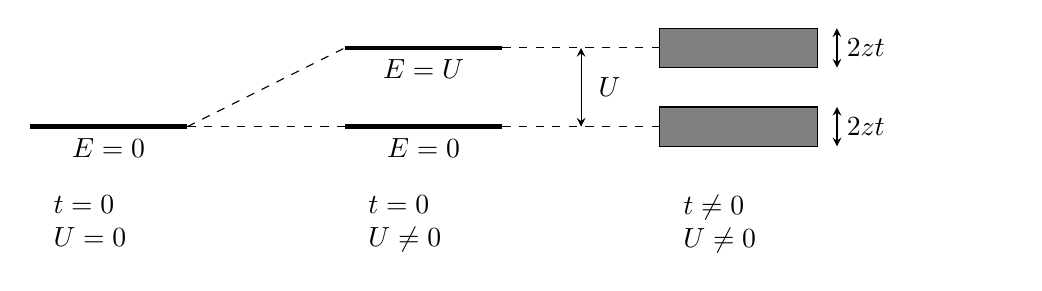
\begin{tikzpicture}
		\draw[level] (0,0) -- node[below] {$ E = 0 $} (2,0);
		\draw[connect] (2, 0) -- node{} (4,0);
		\draw[level] (4,0) -- node[below] {$ E = 0 $} (6,0);
		\draw[connect] (6, 0) -- node{} (8,0);
		\filldraw [gray, draw = black] (8,-0.25) rectangle (10,0.25);
		\draw[arrow] (10.25, -0.25) -- (10.25, 0.25);
		\node[label, right] at (10.25, 0) {$ 2zt $};
		\draw[connect] (2, 0) -- node{} (4,1);
		\draw[level] (4,1) -- node[below] {$ E = U $} (6,1);
		\draw[connect] (6, 1) -- node{} (8,1);
		\filldraw [gray, draw = black] (8,1-0.25) rectangle (10,1.25);
		\draw[arrow] (10.25, 1-0.25) -- (10.25, 1.25);
		\node[label, right] at (10.25, 1) {$ 2zt $};
		
		\draw[arrow] (7,0) -- (7,1);
		\node[label, right] at (7.1, 0.5) {$ U $};
		
		\node[label, below] at (1.3,-0.75) {$ t = 0 $ \\ $ U=0 $};
		\node[label, below] at (5.3,-0.75) {$ t = 0 $ \\ $ U \ne 0 $};
		\node[label, below] at (9.3,-0.75) {$ t \ne 0 $ \\ $ U \ne 0 $};
	\end{tikzpicture}
	\caption{Degenerate bands split into two in presence of electron-electron interaction, and each band further broadens when electrons are allowed to hop.}\label{fig:splitting}
\end{figure}

It is to be noted here that there is a competition between $ t $ and $ U $. While $ U $ tries to separate the high and low energy states, causing the system to acquire insulator-like nature $ T $ tries to bring them closer, making the system more metallic. At a critical value of $ U_{cr} \approx zt $, the bands start splitting. This is called the Mott-Hubbard transition. The large $ U $ regime causes the formation of distinct Hubbard sub-bands at half-filling and is well within the insulating phase. In this phase, the motion of the electrons now become correlated as electrons try to avoid double occupancy.

In order to treat such systems, we will develop an effective Hamiltonian which filters out the high energy states, leaving us only with the states lying in the lowest Hubbard sub-band.

\section{Classification of hopping events}
We will first separate the Hamiltonian into three parts: parts which do not change the energy of the system by preserving the number of double occupancies, and parts which change the energy by altering the number of double occupancies. In order to filter them, we need to first segregate our basis with respect to the hopping events.

Let us first define a set of local projection operators of the form $ \hat{P}_{i a} = \op{a}_{i} $ which returns an eigenvalue $ 1 $ when the site $ i $ has the occupation $ \ket{a}_i $ as shown in section \ref{sec:spectrum}, otherwise returns 0. Explicitly, the four possible operators are
\begin{align}\label{eqn:projectors}
	\nonumber
	\hat{P}_{j 0} &= \op{0}_j = (1 - \hat{n}_{i, \uparrow})(1 - \hat{n}_{i, \downarrow})\\
	\nonumber
	\hat{P}_{j \uparrow} &= \op{\uparrow}_j = \hat{n}_{i, \uparrow} (1 - \hat{n}_{i, \downarrow})\\
	\nonumber
	\hat{P}_{j \downarrow} &= \op{\downarrow}_j = \hat{n}_{i, \downarrow} (1 - \hat{n}_{i, \uparrow})\\
	\hat{P}_{j d} &= \op{d}_j = \hat{n}_{i, \uparrow} \hat{n}_{i, \downarrow}
\end{align}
These operators allow us to check whether a state has a given configuration or not.

Consider two sites $ i $ and $ j $ in a system. Suppose, we only want to consider the hopping that starts from a  causes a $ \uparrow $ particle to hop from a singly-occupied $ i $ and make $ j $ doubly occupied after hopping. We can perform these checks with the projectors defined above before and after the hopping and the hopping term now becomes:
\begin{align}
	\hat{P}_{j, d} c^{\dagger}_{j, \uparrow} c_{i, \uparrow} \hat{P}_{i, \uparrow} = \hat{n}_{j, \uparrow}\hat{n}_{j, \downarrow} c^{\dagger}_{j, \uparrow} c_{i, \uparrow} \hat{n}_{i, \uparrow} (1 - \hat{n}_{i, \downarrow}) = \hat{n}_{j, \downarrow} c^{\dagger}_{j, \uparrow} c_{i, \uparrow} (1 - \hat{n}_{i, \downarrow})
\end{align}

This is called a projected hopping, in the sense that this is only a projection of a part of the total space of states that can be created by this hopping.

We see that the above hopping increases the number of doubly occupied sites by one. Collecting all such terms together, we can write the part of the Hamiltonian which increases the number of double occupations in the system by one:

\begin{align}\label{eqn:Ht+}
H^{+}_{t} = -t \sum_{\langle i, j \rangle} \sum_{\sigma} \left[ \hat{n}_{i, -\sigma} c^{\dagger}_{i, \sigma} c_{j, \sigma} (1 - \hat{n}_{j, -\sigma}) + h.c.\right]
\end{align}

Similarly, the Hamiltonian for processes which decrease the number of double occupations is given as
\begin{align}\label{eqn:Ht-}
	H^{-}_{t} = -t \sum_{\langle i, j \rangle} \sum_{\sigma} \left[ (1 - \hat{n}_{i, -\sigma}) c^{\dagger}_{i, \sigma} c_{j, \sigma} \hat{n}_{j, -\sigma} + h.c.\right]
\end{align}

There can also be processes which preserve the number of doubly-occupied states, where we check whether both the initial and final states are doubly- \textbf{or} singly-occupied. The Hamiltonian for such processes can be shown to be

\begin{align}\label{eqn:Ht0}
	H^{0}_{t} = -t \sum_{\langle i, j \rangle} \sum_{\sigma} \left[ (1 - \hat{n}_{i, -\sigma}) c^{\dagger}_{i, \sigma} c_{j, \sigma} (1 - \hat{n}_{j, -\sigma}) + \hat{n}_{i, -\sigma} c^{\dagger}_{i, \sigma} c_{j, \sigma} \hat{n}_{j, -\sigma} + h.c.\right]
\end{align}

Combining these three, we can write the band Hamiltonian as
\begin{align}\label{eqn:hband}
	H_{\mathrm{band}} = H^{+}_{t} + H^{-}_{t} + H^{0}_{t}
\end{align}

The action of $ H^{\pm}_{t} $ can change the energy of the system and thus, transfers electrons from one sub-band to another. On the other hand, $ H^{0}_{t} $ preserves the energy of a state under its action and thus, restricts an electron to its band. As a result, overall, $ H_{\mathrm{band}} $, responsible for the hopping of electrons between sites, leads to a mixing of states between two bands. Also, this results in all hopping not being equally probable, depending on the local environment of the electron. This gives a many-body nature to the kinetic energy part of the Hamiltonian.

\chapter{Schrieffer-Wolff transformations and Hubbard operators}
\section{Schrieffer-Wolff transformations}
Equation \eqref{eqn:hband} shows that $ H^{\pm}_{t} $ mixes states from different bands. In order to avoid that, we can form suitable linear combinations of the basis states. We can introduce a canonical transformation called the Schrieffer-Wolff transformations. The full Hamiltonian is given as
\begin{align}
H = H_{\mathrm{band}} + H_U
\end{align}

Then, the transformed effective Hamiltonian is
\begin{align}
\nonumber
H_{\mathrm{eff}} &= \exp(\I S) H \exp(-\I S)\\
\nonumber
&= H \I \comm{S}{H} + \frac{\I^2}{2} \comm{S}{\comm{S}{H}} + \dots\\
&= H_U + H_{\mathrm{band}} + \I \comm{S}{H_U} + \I \comm{S}{H_{\mathrm{band}}} + \frac{\I^2}{2} \comm{S}{\comm{S}{H_{\mathrm{band}}  }} + \dots
\end{align}

where $ S $ is a suitably chosen generator for the transformation such that $ H_{\mathrm{eff}} $ no longer connects the different bands.

In order to guess the form of $ S $, we can try to commute one part of $ H^{+}_{t} $ with $ H_U $.
\begin{align}
\nonumber
&\comm{\hat{n}_{i, \downarrow} c^{\dagger}_{i,\uparrow} c_{j, \uparrow} (1 - \hat{n}_{j, \downarrow})}{ \hat{n}_{i, \uparrow} \hat{n}_{i, \downarrow} }\\
\nonumber
=&\,
\hat{n}_{i, \downarrow} c^{\dagger}_{i,\uparrow} c_{j, \uparrow} (1 - \hat{n}_{j, \downarrow}) \hat{n}_{i, \uparrow} \hat{n}_{i, \downarrow}
-
\hat{n}_{i, \uparrow} \hat{n}_{i, \downarrow} \hat{n}_{i, \downarrow} c^{\dagger}_{i,\uparrow} c_{j, \uparrow} (1 - \hat{n}_{j, \downarrow})\\
\nonumber
=&\,
\hat{n}_{i, \downarrow}\hat{n}_{i, \downarrow} c^{\dagger}_{i,\uparrow}\hat{n}_{i, \uparrow} c_{j, \uparrow} (1 - \hat{n}_{j, \downarrow})  
-
\hat{n}_{i, \uparrow} \hat{n}_{i, \downarrow} \hat{n}_{i, \downarrow} c^{\dagger}_{i,\uparrow} c_{j, \uparrow} (1 - \hat{n}_{j, \downarrow})\\
\nonumber
=&\,
\hat{n}_{i, \downarrow} c^{\dagger}_{i, \downarrow} c_{i, \downarrow} c^{\dagger}_{i, \uparrow} c^{\dagger}_{i, \uparrow} c_{i, \uparrow} c_{j, \uparrow} (1 - n_{j, \downarrow})
-
\hat{n}_{i, \uparrow} \hat{n}_{i, \downarrow} \hat{n}_{i, \downarrow} c^{\dagger}_{i,\uparrow} c_{j, \uparrow} (1 - \hat{n}_{j, \downarrow})\\
\nonumber
=&\,
-n_{i, \downarrow} c^{\dagger}_{i, \uparrow} c_{j, \uparrow} (1 - n_{j, \downarrow})
+
\hat{n}_{i, \uparrow} \hat{n}_{i, \downarrow} \hat{n}_{i, \downarrow} c^{\dagger}_{i,\uparrow} c_{j, \uparrow} (1 - \hat{n}_{j, \downarrow})
-
\hat{n}_{i, \uparrow} \hat{n}_{i, \downarrow} \hat{n}_{i, \downarrow} c^{\dagger}_{i,\uparrow} c_{j, \uparrow} (1 - \hat{n}_{j, \downarrow})\\
=&\,
-n_{i, \downarrow} c^{\dagger}_{i, \uparrow} c_{j, \uparrow} (1 - n_{j, \downarrow})
\end{align}

From this, we can conclude that
\begin{align}
\comm{H^{\pm}_{t}}{H_U} = \mp U H^{\pm}_{t}
\end{align}

Therefore, the form of the transformation can now be guessed as
\begin{align}\label{eqn:swtransform}
S = - \frac{\I}{U} \left( H^{+}_{t} - H^{-}_{t} \right)
\end{align}

Then,
\begin{align}
\nonumber
H_{\mathrm{eff}} =& H_U + H_{\mathrm{band}} - \left( H^{+}_{t} - H^{-}_{t} \right) + \frac{2}{U} \comm{H^{+}_{t}}{H^{-}_{t}} - \frac{\I}{2} \comm{S}{\comm{H^{+}_{t}}{H^{-}_{t}}} + \order{\frac{t^3}{U}}\\
\nonumber
=& H_U + H^{0}_{t} + \frac{2}{U} \comm{H^{+}_{t}}{H^{-}_{t}} - \frac{1}{U} \comm{H^{+}_{t}}{H^{-}_{t}} + \order{\frac{t^3}{U}}\\
=& H_U + H^{0}_{t} + \frac{1}{U} \comm{H^{+}_{t}}{H^{-}_{t}} + \order{\frac{t^3}{U}}
\end{align}

The commutator $ \comm{H^{+}_{t}}{H^{-}_{t}} $ can now be calculated by introducing Hubbard operators.

\section{Hubbard Operators}
A Hubbard operator takes a site from occupation state $ \ket{a}_i $ to $ \ket{b}_i $ and is of the form
\begin{align}
X^{b \leftarrow a}_{j} = \op{b}{a}_i
\end{align}

The definition readily admits the property that
\begin{align}
\left( X^{b \leftarrow a}_{j}\right) ^{\dagger} = X^{a \leftarrow b}_{j}
\end{align}

Using the same logic as the projection operators, the Hubbard operators can be expressed in terms of the creation, annihilation and number operators as
\begin{align}
X^{\sigma \leftarrow 0}_{j} &= c^{\dagger}_{j, \sigma} (1 - \hat{n}_{j, -\sigma})\\
X^{0 \leftarrow \sigma}_{j} &= c_{j, \sigma} (1 - \hat{n}_{j, -\sigma})\\
X^{d \leftarrow \sigma}_{j} &= \eta(\sigma) c^{\dagger}_{j, \sigma} \hat{n}_{j, \sigma} \\
X^{\sigma \leftarrow d}_{j} &= \eta(\sigma) c_{j, \sigma} \hat{n}_{j, \sigma}
\end{align}

where
\begin{align}
\eta(\sigma) = \left.
\begin{cases}
+1 & \text{for} \sigma = \uparrow\\
-1 & \text{for} \sigma = \downarrow\\
\end{cases}
\right\}
\end{align}

The $ \eta(\sigma) $ is required to maintain the convention of $ \ket{d}_i $.

Using this, the product of two Hubbard operators can be defined as
\begin{align}
X^{c \rightarrow f}_{j} X^{b \rightarrow a}_{j} = \delta_{bf} X^{c \leftarrow a}_{j}
\end{align}

The commutator is given as
\begin{align}
\comm{X^{b \leftarrow a}_{i}}{X^{d \leftarrow c}_{j}} = \delta_{ij} \left( \delta_{ab} X^{b \leftarrow c}_{j} - \delta_{bc} X^{d \leftarrow a}_{j} \right)
\end{align}

Also, we can get the relation
\begin{align}
c^{\dagger}_{j, \sigma} = X^{\sigma \leftarrow 0}_j + \eta(\sigma) X^{d \leftarrow -\sigma}_{j}
\end{align}

Using all in the above properties, from equations \eqref{eqn:Ht+}, \eqref{eqn:Ht-} and \eqref{eqn:Ht0}, we get
\begin{align}
\label{eqn:Ht+hubbard}
H^{+}_{t} &= -t \sum_{\langle i, j \rangle} \sum_{\sigma} \eta(\sigma) \left[ X^{d \leftarrow -\sigma} X^{0 \leftarrow \sigma}_j + h.c. \right]\\
\label{eqn:Ht-hubbard}
H^{-}_{t} &= -t \sum_{\langle i, j \rangle} \sum_{\sigma} \eta(\sigma) \left[ X^{\sigma \leftarrow 0} X^{-\sigma \leftarrow d}_j + h.c. \right]\\
H^{0}_{t} &= -t \sum_{\langle i, j \rangle} \sum_{\sigma} \left[ X^{\sigma \leftarrow 0}_{i} X^{0 \leftarrow \sigma}_{j} + h.c. \right]
\end{align}

\chapter{The t-J model}
\section{Large U limit}
In the t-J model, we only consider the low energy subspace. As a result, we can immediately disregard the $ H_U $ as well as the state $ \ket{d}_i $ from the basis. As a result, the zero-th order hopping only includes the part of $ H^{0}_{t} $ which maintain the number of single occupancies.
\begin{align}
H^{0}_{t} = -t \sum_{\langle i, j \rangle} \sum_{\sigma} \left[ X^{\sigma \leftarrow 0}_i X^{0 \leftarrow \sigma}_j + h.c. \right]
\end{align}

\section{Two-site terms}
First, we consider hopping between only two adjacent sites, up to all orders.

For evaluating $ \comm{H^{+}_{t}}{H^{-}_{t}} $, we neglect the term $ H^{+}_{t} H^{-}_{t} $ as the its action all the single-occupancy states automatically destroys them. Hence,
\begin{align}
\nonumber
\comm{H^{+}_{t}}{H^{-}_{t}} =&  -H^{-}_{t} H^{+}_{t}\\
\nonumber
=& -t^2 \sum_{\sigma} \sum_{\sigma'} \eta(\sigma) \eta(\sigma') X^{\sigma' \leftarrow 0}_j X^{-\sigma' \leftarrow d}_i X^{d \rightarrow-\sigma'}_i X^{0 \rightarrow \sigma}_j\\
\nonumber
=& -t^2 \sum_{\sigma} \sum_{\sigma'} \eta(\sigma) \eta(\sigma')  X^{-\sigma' \leftarrow -\sigma}_i X^{\sigma' \leftarrow \sigma}_j\\
=& -t^2 \sum_{\sigma}\left[ X^{-\sigma \leftarrow -\sigma}_i  X^{\sigma \leftarrow \sigma}_j + X^{\sigma \leftarrow -\sigma}_i  X^{-\sigma \leftarrow \sigma}_j \right]
\end{align}

The first term only consists of diagonal operators that do not alter spin. The spin-operator has a similar behaviour:

\begin{align}
S^{z}_{i} \ket{\sigma}_i = \frac{1}{2} \eta(\sigma) \ket{\sigma}_i
\end{align}

This gives

\begin{align}
X^{\sigma \leftarrow \sigma} = \eta(\sigma) S^{z}_{i} + \frac{1}{2}
\end{align}

The diagonal part of the operator can now be reduced to
\begin{align}\label{eqn:2sitediag}
-t^2 \sum_{\sigma}  X^{-\sigma \leftarrow -\sigma}_i  X^{\sigma \leftarrow \sigma}_j = 2 t^2 \left[ S^{z}_{i} S^{z}_{j} - \frac{1}{4} \right]
\end{align}

Now, we know, the spin-raising or lowering operators act as
\begin{align}
S^{+}_{i} \ket{\downarrow}_i &= \ket{\uparrow}_i\\
S^{-}_{i} \ket{\uparrow}_i &= \ket{\downarrow}_i
\end{align}

Comparing with the action of the Hubbard operators, we can write
\begin{align}
X^{\uparrow \leftarrow \downarrow}_{i} &= S^{+}_{i}\\
X^{\downarrow \leftarrow \uparrow}_{i} &= S^{-}_{i}
\end{align}

Then,
\begin{align}\label{eqn:2siteoffdiag}
\nonumber
&t^2 \left[ X^{\uparrow \leftarrow \downarrow}_{i} X^{\downarrow \leftarrow \uparrow}_{j} + X^{\downarrow \leftarrow \uparrow}_{j} X^{\uparrow \leftarrow \downarrow}_{i} \right]\\
\nonumber
=& t^2 \left[ S^{+}_{i}S^{-}_{j} + S^{-}_{i}S^{+}_{j}  \right]
\end{align}

This operator returns 0 if the two adjacent sites have parallel spins. If the two spins are anti-parallel, they are exchanged. This already indicates a correlated hopping behaviour.

Also, know that
\begin{align}
S^{\pm}_i = S^{x}_i \pm \I S^{y}_i
\end{align}

Putting this in \eqref{eqn:2siteoffdiag}, we get
\begin{align}\label{eqn:offdfinal}
t^2 \left[ S^{+}_{i}S^{-}_{j} + S^{-}_{i}S^{+}_{j} \right] = 2 t^2 \left[ S^{x}_i \cdot S^{x}_j + S^{y}_i \cdot S^{y}_j \right]
\end{align}

Combining \eqref{eqn:2sitediag} and \eqref{eqn:offdfinal}, we get
\begin{align}
\comm{ {H^{+}_{t}}_{i,j} }{ {H^{-}_{t}}_{i,j} } = 2 t^2 \left[ \vec{S_{i}} \cdot \vec{S_{j}} - \frac{1}{4} \hat{n}_i \hat{n}_j \right]
\end{align}

The final Hamiltonian is now given as:
\begin{align}\label{eqn:Htj}
\nonumber
H_{\mathrm{t-J}} =& -t^2 \sum_{\langle i,j } \sum_\sigma\left[ (1 - \hat{n}_{i, -\sigma}) c^{\dagger}_{i, \sigma} c_{j, \sigma} (1 - \hat{n}_{j, -\sigma}) + \hat{n}_{i, -\sigma} c^{\dagger}_{i, \sigma} c_{j, \sigma} \hat{n}_{j, -\sigma} + h.c. \right]\\ &+ \frac{4 t^2}{U} \left[ \vec{S_{i}} \cdot \vec{S_{j}} - \frac{1}{4} \hat{n}_i \hat{n}_j \right] + \text{3-site terms}
\end{align}

\section{Three-site terms}
We will now consider hopping between three adjacent sites. In the first case, we assume that three sites contain two particles of opposite spins, with an initial configuration of $ \ket{0\uparrow\downarrow} $.

The process arising from $ \comm{ {H^{+}_{t}}_{i,j} }{ {H^{-}_{t}}_{j,k} } $ occurs in the following way:
\begin{align*}
\ket{0\uparrow\downarrow} \xrightarrow{ {H^{+}_{t}}_{j,k} } \ket{0d0} &\xrightarrow{A:\, {H^{-}_{t}}_{i,j}} \ket{\uparrow \downarrow 0}\\
&\xrightarrow{B:\, {H^{-}_{t}}_{i,j}} \ket{\downarrow \uparrow  0}
\end{align*}

Defining the projected hopping operator
\begin{align}
\tilde{c}^{\dagger}_{i,\sigma} = c^{\dagger}_{i,\sigma} (1 - \hat{n}_{i, -\sigma})
\end{align}

We get
\begin{align}
\nonumber
H^{A}_{\mathrm{3-site}} &= -\frac{t^2}{U} \sum_{\langle i,j } \sum_\sigma \left[ c^{\dagger}_{i, \sigma} (1 - \hat{n}_{i, -\sigma}) \hat{n}_{j, -\sigma} c_{k, \sigma} (1 - \hat{n}_{k, -\sigma}) + h.c.\right]\\
&=
-\frac{t^2}{U} \sum_{\langle i,j } \sum_\sigma \left[ \tilde{c}^{\dagger}_{i, \sigma} \hat{n}_{j, -\sigma} \tilde{c}_{k, \sigma} + h.c. \right]
\end{align}

Similarly,
\begin{align}
\nonumber
H^{B}_{\mathrm{3-site}} &= 
-\frac{t^2}{U} \sum_{\langle i,j } \sum_\sigma \left[ \tilde{c}^{\dagger}_{i, \sigma} \tilde{c}^{\dagger}_{j, \sigma} \tilde{c}_{j, -\sigma} \tilde{c}_{k, \sigma} + h.c. \right]
\end{align}

Thus, up to $ \order{\frac{t}{U}} $, we have successfully separated the bands. This allows us to look at the low energy sub-bands only, without worrying about the high energy spectrum.

Next, if we examine the contributions of the $ \I \comm{S}{H^{0}_{t}} $ term, we will find that after two hops, the system moves from a singly occupied state to a doubly occupied state. However, since these terms are of $ \order{\frac{t^2}{U}} $, we will neglect them. These bands can be separated by adding another transformation, however, higher order bands will still remain mixed. In fact, it is impossible to separate all bands in a finite number of steps.

\chapter{Solving the Heisenberg model using the t-J model}
\section{Hesisenberg model as a special case of t-J model}
At a large $ U $ limit with $ n = 1 $, the t-J model becomes the Heisenberg model. At half-filling, the system lacks pairs or holes once we neglect double occupations. If we neglect the density-density term, the Hamiltonian for the Heisenberg model is given as
\begin{align}
H = \frac{4t^2}{U} \sum_{\langle i,j \rangle} \vec{S_{i}} \cdot \vec{S_{j}}
\end{align}
Thus, the Hamiltonian only acts on spin states, like the t-J model Hamiltonian.

\section{Density calculation for a site}
To see whether the t-J model successfully captures the behaviour of this system, let us calculate the density of a doubly occupied site in the large $ U $ limit. We will do this by performing a Schrieffer-Wolff transformation on the ground state $ \ket{\psi} $ of the Hubbard model and transform it to the ground state of the effective Hamiltonian, $ \ket{\tilde{\psi}} = \exp(\I S) \ket{\psi} $.

\begin{align}
\nonumber
n_d &= \expval{ \hat{n}_{j,\uparrow} \hat{n}_{j,\downarrow} }{\psi}\\
\nonumber
&= \expval{X^{d \leftarrow d}_{j}}{\psi}\\
\nonumber
&= \expval{\exp(-\I S)\exp(\I S)X^{d \leftarrow d}_{j}\exp(-\I S)\exp(\I S)}{\psi}\\
\nonumber
&= \expval{\exp(\I S)X^{d \leftarrow d}_{j}\exp(-\I S)}{\tilde{\psi}}\\
\nonumber
&= \expval{\left( 1 + \I S - \frac{1}{2} S^2 + \cdots \right) X^{d \leftarrow d}_{j} \left( 1 + \I S - \frac{1}{2} S^2 + \cdots \right) }{\tilde{\psi}}\\
\nonumber
&= \expval{X^{d \leftarrow d}_{j}}{\tilde{\psi}} + \I \expval{S X^{d \leftarrow d}_{j} - X^{d \leftarrow d}_{j} S}{\tilde{\psi}} + \expval{S X^{d \leftarrow d}_{j} S}{\tilde{\psi}} + \cdots\\
&= \expval{X^{d \leftarrow d}_{j}}{\tilde{\psi}} + \I \expval{S X^{d \leftarrow d}_{j}}{\tilde{\psi}} - \I \expval{X^{d \leftarrow d}_{j} S}{\tilde{\psi}} + \expval{S X^{d \leftarrow d}_{j} S}{\tilde{\psi}} + \cdots
\end{align}

As $ \ket{\tilde{\psi}} $ is the ground state of the effective Hamiltonian, all high energy states are to eliminated and therefore,
\begin{align}
X^{d \leftarrow d}_{j}\ket{\tilde{\psi} }= 0
\end{align}

Then,
\begin{align}
\nonumber
n_d 
=&
\expval{S X^{d \leftarrow d}_{j} S}{\tilde{\psi}}\\
=&
\frac{1}{U^2}\expval{\left(H^{+}_t - H^{-}_{t}\right)X^{d \leftarrow d}_{j}\left(H^{+}_t - H^{-}_{t}\right)}
\end{align}

Now, using the fact that we are considering only single occupancy states, the double-occupancy lowering part of the Hamiltonian destroys the ground state upon acting on it. Substituting equations \eqref{eqn:Ht+hubbard} and \eqref{eqn:Ht-hubbard} into this and following the same steps as deriving \eqref{eqn:Htj}, this gives us
\begin{align}
\nonumber
n_d =&
2z\frac{t^2}{U^2} \expval{\frac{1}{4} - \vec{S_{1}}\cdot\vec{S_{2}}}{\tilde{\psi}}
\end{align}

where $ z $ is the coordination number of the sites. As expected, the density at each site is proportional to the spin-correlation operator.

Similarly, we can calculate the band energy term for the interaction energy density:
\begin{align}
\frac{1}{L}\expval{H_U}{\psi} = \frac{t^2}{U} \left[1 - 4 \expval{\vec{S_{1}}\cdot\vec{S_{2}}}{\tilde{\psi}} \right]
\end{align}

For the band energy density,
\begin{align}
\frac{1}{L}\expval{H_\mathrm{band}}{\psi} = 4\frac{t^2}{U} \left[1 - 4 \expval{\vec{S_{1}}\cdot\vec{S_{2}}}{\tilde{\psi}} \right]
\end{align}

Adding these two, we get
\begin{align}
\frac{1}{L}\expval{H}{\psi} = -2\frac{t^2}{U}  \expval{\vec{S_{1}}\cdot\vec{S_{2}} - \frac{1}{4}}{\tilde{\psi}}
\end{align}

\end{document}

